\documentclass[a4paper,12pt]{article}
\usepackage[a4paper,top=1.3cm,bottom=2cm,left=1.5cm,right=1.5cm,marginparwidth=0.75cm]{geometry}
\usepackage{setspace}
\usepackage{cmap}		
\usepackage{amsmath,amsfonts,amssymb,amsthm,mathtools} 			
 				
\usepackage[T2A]{fontenc}			
\usepackage[utf8]{inputenc}			
\usepackage[english,russian]{babel}
\usepackage{multirow}
\usepackage{graphicx}
\usepackage{wrapfig}
\usepackage{tabularx}
\usepackage{float}
\usepackage{longtable}
\usepackage{hyperref}
\hypersetup{colorlinks=true,urlcolor=blue}
\usepackage[rgb]{xcolor}
\usepackage{icomma} 
\usepackage{euscript}


\DeclareMathOperator{\sgn}{\mathop{sgn}}
\newcommand*{\hm}[1]{#1\nobreak\discretionary{}
	{\hbox{$\mathsurround=0pt #1$}}{}}


\title{\textbf{Изготовление дифракционной решетки с помощью
фотолитографии. Измерение длины волны лазера.}}
\author{Лавыгин Кирилл}
\date{\today}


\begin{document}
	
	\maketitle
	
	\section*{Аннотация}
	В ходе работы были изготовлена дифракционные решетки напылением алюминия на оксидированную и неоксидированную кремниевые подложки. С помощью изготовленных решеток была измерена длина волны лазера.

\section*{Оборудование}
Установка экспонирования, фотошаблон, центрифуга для нанесения резиста, HotPlate для его сушки, установка термического напыления ВУП-5, оптический и электронный микроскопы, лазер, экран с миллиметровой бумагой, рулетка.

\section*{Изготовление дифракционных решёток}
Процесс изготовления образцов состоял из следующих этапов:

\begin{enumerate}
    \item \textbf{Подготовка подложек} \\
    Для изготовления образцов были использованы подложки из чистого и оксидированного кремния. Исходный материал был аккуратно поломан (ещё точнее это можно сделать скрайбером) на небольшие части, пригодные по размеру для создания образцов.

    \item \textbf{Нанесение резиста} \\
    Перед нанесением резиста подложки необходимо очистить – обезжирить ацетоном и ненадолго поместить в ультразвуковую ванну. После промывания в ацетоне подложки помещаются на центрифугу, на них наносится несколько капель резиста (в работе был использован позитивный резист S1811). Вращение центрифуги необходимо для равномерного растекания резиста, процесс происходит на скорости 6000 об./мин. в течение 20 с. Далее производится сушка на HotPlate в течение 3 минут при температуре $T = 95^\circ$C. В результате получаем твердую пленку резиста на поверхности образца.

    \item \textbf{Экспонирование} \\
    Экспонирование резиста осуществлялось методом контактной фотолитографии с использованием лампы длиной волны 365 нм в течение 10 секунд. При экспонировании был использован негативный фотошаблон, изготовленный ранее с помощью электронной литографии по предварительно созданным чертежам и представляющий собой последовательность полос-щелей шириной $b = 100$ мкм и периодом $d = 200$ нм.

    \item \textbf{Проявление} \\
    Проявление было проведено в слабой щёлочи (0.8\% раствор КОН). Засвеченные участки вымываются быстрее незасвеченных, однако передержать образцы в растворе нельзя, так как будет происходить удаление засвеченного резиста, что приведет к деффектам. По отработанной технологии проявление проводится в течение 10 секунд, затем образцы промываются водой и помещаются на центрифугу на сушку. Далее была произведена проверка образцов на оптическом микроскопе.

    \item \textbf{Нанесение плёнки} \\
    На проявленный резист была нанесена алюминиевая плёнка методом термического напыления на установке ВУП-5. При термическом испарении нельзя регулировать толщину плёнки по скорости (скорость непостоянна), однако при использованной нами алюминиевой навеске массой  толщина плёнки получается равной порядка 100 нм.

    \item \textbf{Взрывная литография (Lift-off)} \\
    Удаление резиста с напылённым сверху алюминием производится в органическом растворителе – нами был использован ацетон. На первом этапе резист удалялся по краям подложки, в центре (около решётки) алюминий был удалён при помощи струи ацетона. В завершение изготовленные решётки были промыты водой, а остатки жидкости удалены при помощи центрифуги.
\end{enumerate}

\begin{figure}[h!]
\centering
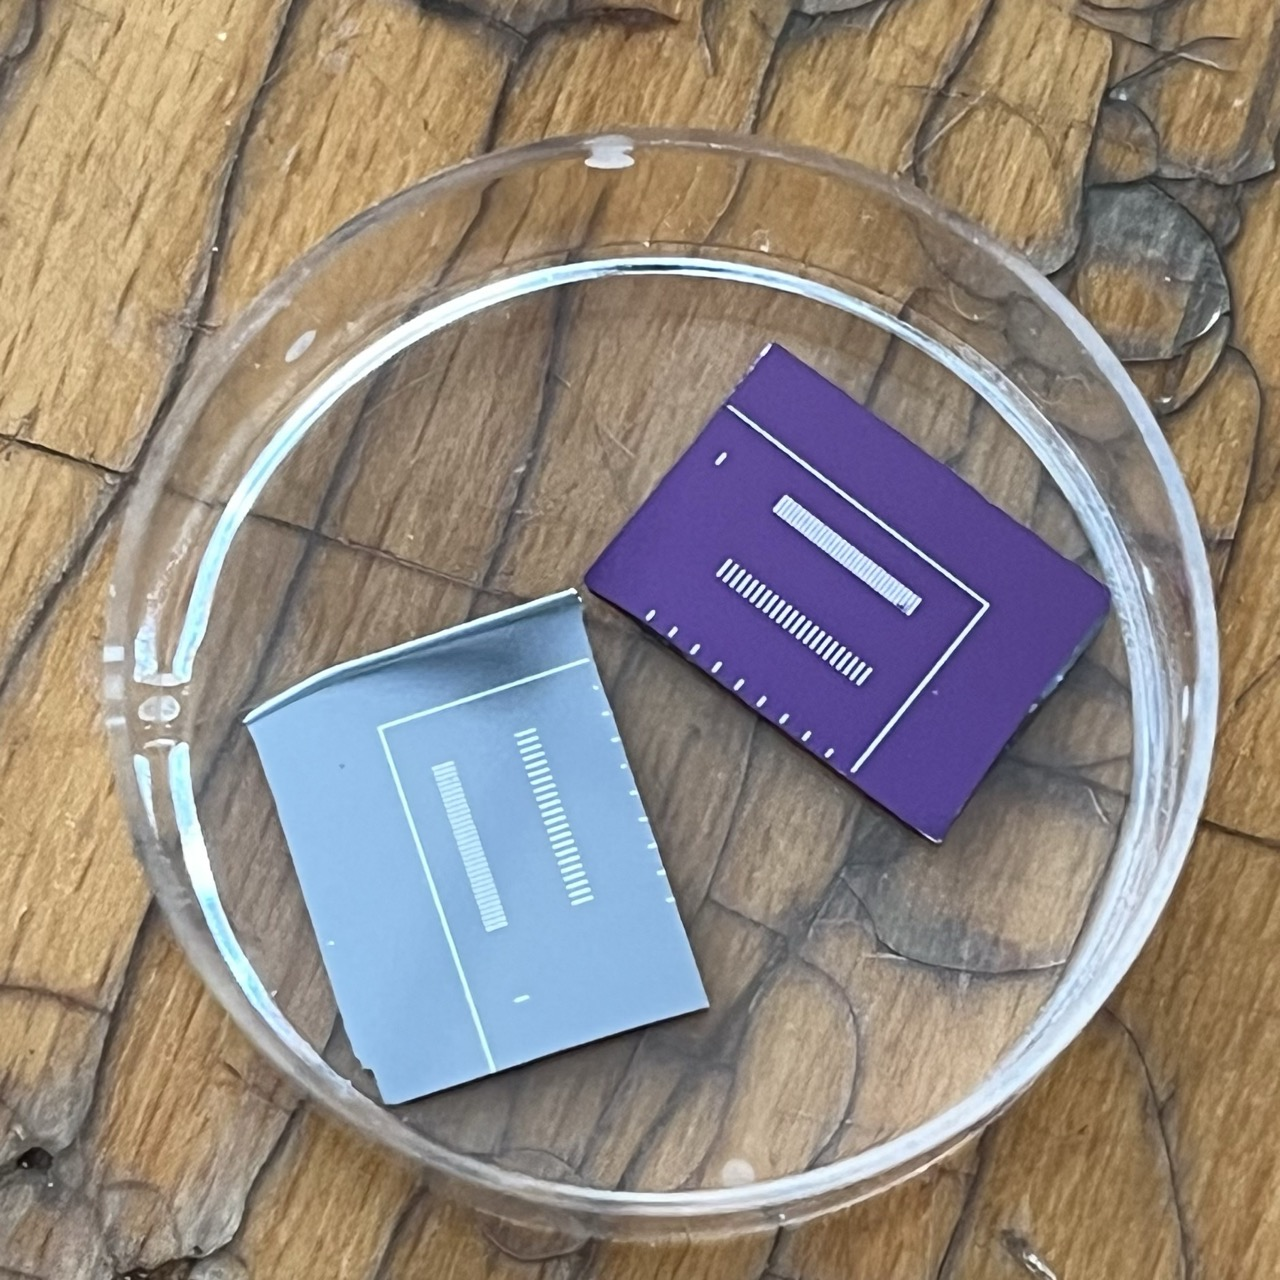
\includegraphics[width=0.5\textwidth]{samps}
\caption{Готовые образцы}
\end{figure}

В результате соблюдения методики изготовления образцов удалось создать дифракционные решётки удовлетворительного качества. В рамках фиксированного техпроцесса наиболее сложным этапом является взрыв, так как тон ребует механической работы и плохо повторяется по инструкции. Образец на оксидированной подложке я взрывал более агрессивно, что лишило его "ушей" на краях, но привело к повреждению части полос (возможно и из-за повреждения резиста). Образец на чистой подложке был взорван более мягко, что привело к появлению заметных "ушей" и обломков пленки.

\begin{figure}[h!]
\centering
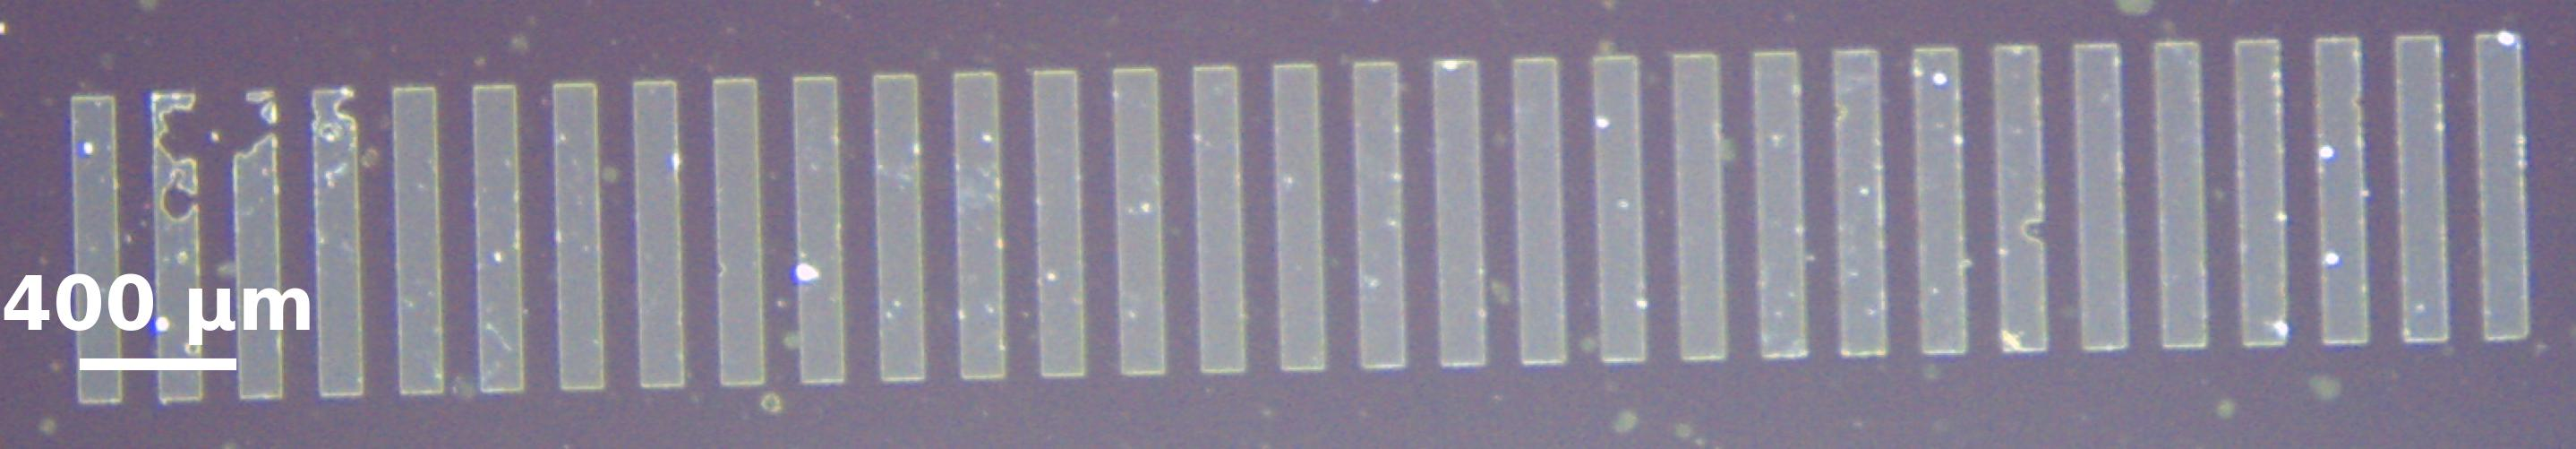
\includegraphics[width=0.8\textwidth]{lavygin_ox_full_scale}
\caption{Фотография образца на оксидированной подложке на оптическом микроскопе}
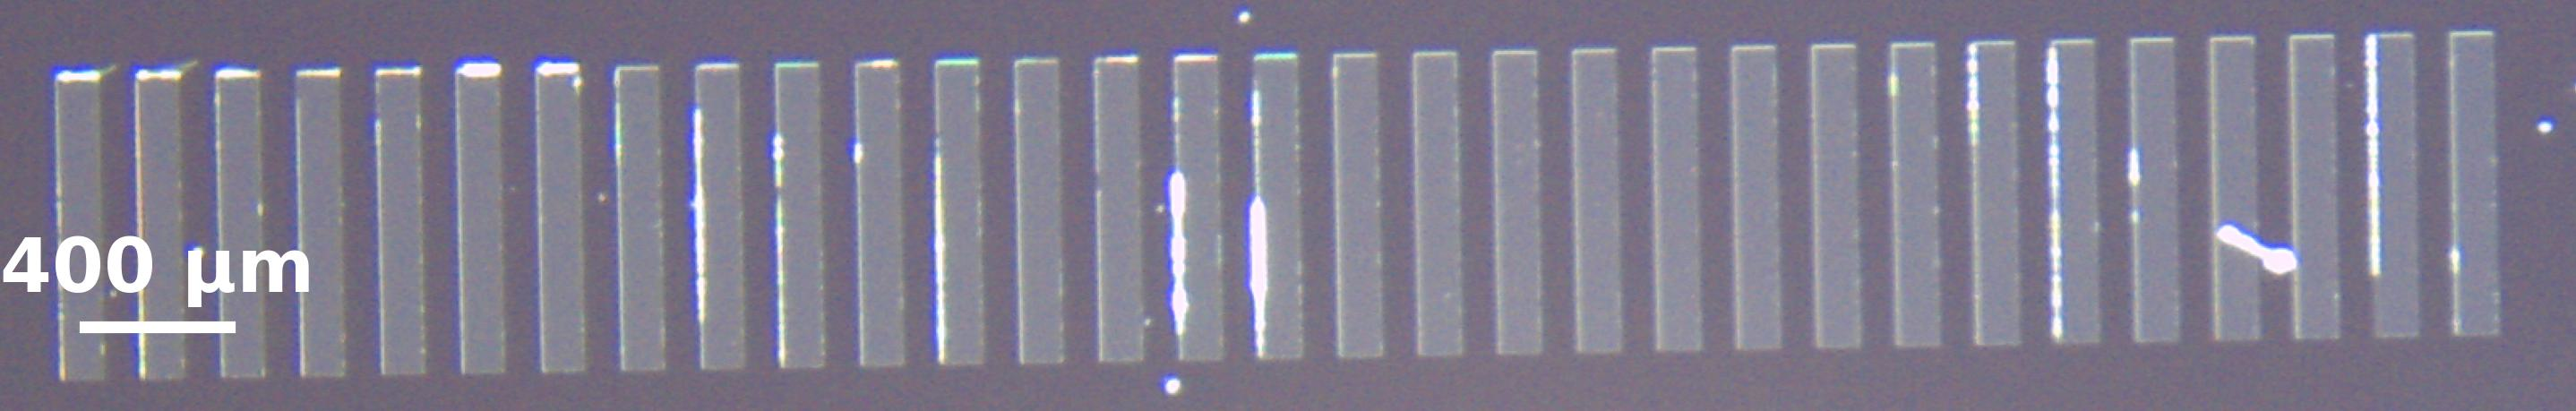
\includegraphics[width=0.8\textwidth]{lavygin_norm_full_scale}
\caption{Фотография образца на чистой подложке на оптическом микроскопе}
\end{figure}

\newpage

\section*{Измерение параметров дифракционной решётки}
Параметры дифракционных решёток изготовленных образцов были измерены с помощью оптического микроскопа и с помощью сканирующего электронного микроскопа. Фотографии представлены в Приложении.

Результаты были получены усреднением трех измерений.
\begin{table}[h!]
\centering
\caption{Результаты измерения ширины полосы и периода}
\begin{tabular}{ccc}
\toprule
Тип подложки и микроскопа & Ширина полосы $b$, мкм & Период решётки $d$, мкм \\
\midrule
Шаблон & 100 & 200 \\
СЭМ: Чистая подложка & 92 & 190 \\
ОМ: Чистая подложка  & 101.9 & 200.5 \\
ОМ: Оксидированная подложка & 101.3 & 200.3 \\
\bottomrule
\end{tabular}
\end{table}

Как можно заметить, результаты СЭМ серьезно отличаются от оптических и ожидаемых. Проблема в том, что микроскоп никогда не калибровался, поэтому абсолютные значения полученные на нем, по нашему мнению, не представляют ценности. Единственная полезная информация c СЭМ о структуре - полосы одного могут отличаться по ширине на $\approx1$ мкм. 

В дальнейших расчетах используются измерения с оптического микроскопа
\section*{Моделирование дифракционной картины}
Перед проведением эксперимента рассчитаем дифракционную картину для исследуемой решётки. При отражении света длиной волны $\lambda$ от дифракционной решетки с периодом $d$, состоящей из одинаковых, расположенных на одном и том же расстоянии друг от друга зеркальных полос шириной $b$, интенсивность света как функция угла $\phi = \frac{x}{L}$, отсчитанного от нормали к плоскости решетки, определяется известной формулой:
\[
I = \left( \frac{\sin(\pi b \sin(\phi)/\lambda)}{\pi b \sin(\phi)/\lambda} \right)^2 \cdot \left( \frac{\sin(N\pi d \sin(\phi)/\lambda)}{\pi d \sin(\phi)/\lambda} \right)^2
\]
Здесь $d$ – период решётки; $b$ – ширина полосы; $\lambda$ – длина волны лазера; $N$ – число активных полос дифракционной решётки; $\phi = \frac{x}{L}$ – угол, отсчитанный от нормали к плоскости решётки, где $x$ – координата, отсчитываемая от главного максимума.

В случае исследуемой решётки $2b = d = 200$ мкм; длину волны используемого лазера положим равной $\lambda = 550$ нм; расстояние от решетки до экрана 270 см; пятно лазера порядка 5мм, а значит число полос решётки $N \approx 25$ю
Результаты моделирования представлены на Рис. 4.

\begin{figure}[h!]
\centering
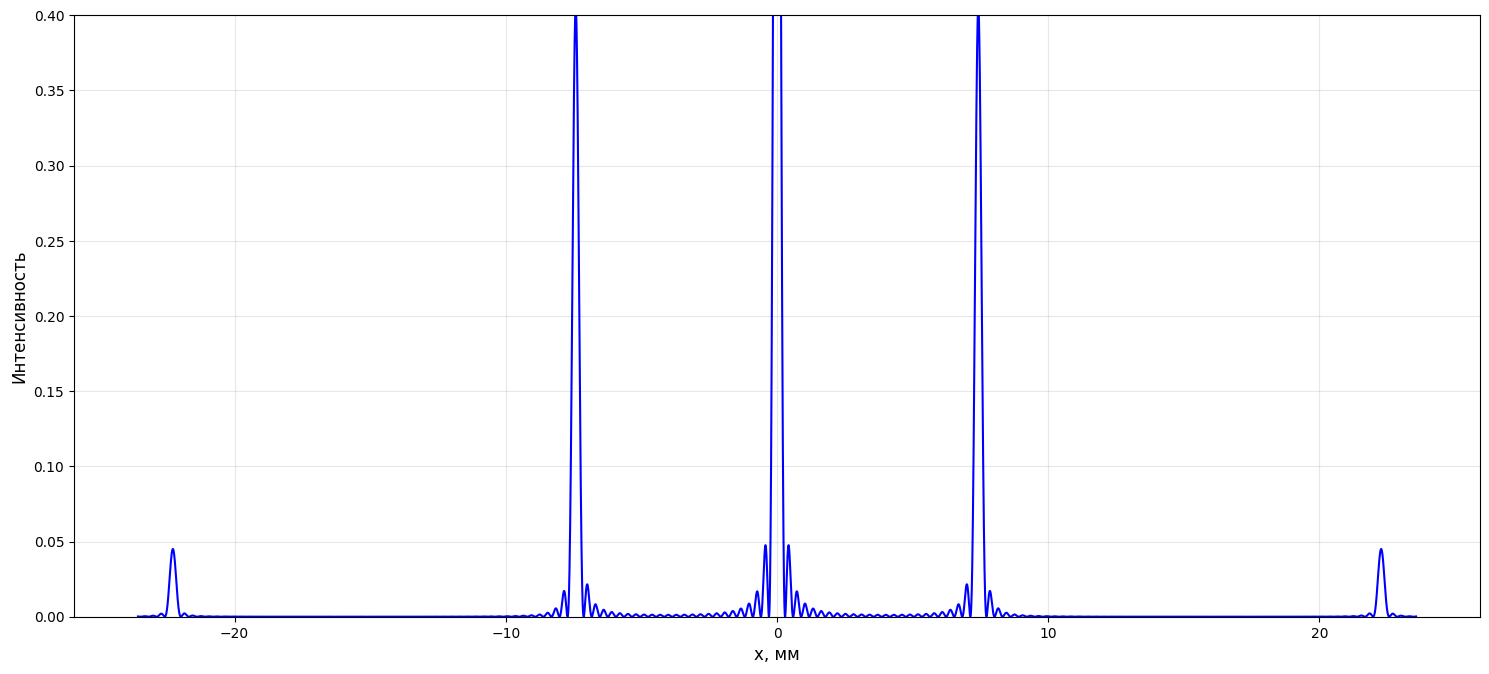
\includegraphics[width=\textwidth]{mod.png}

\caption{Результаты моделирования}
\end{figure}

\newpage

\section*{Эксперимент}

\begin{figure}[h!]
\centering
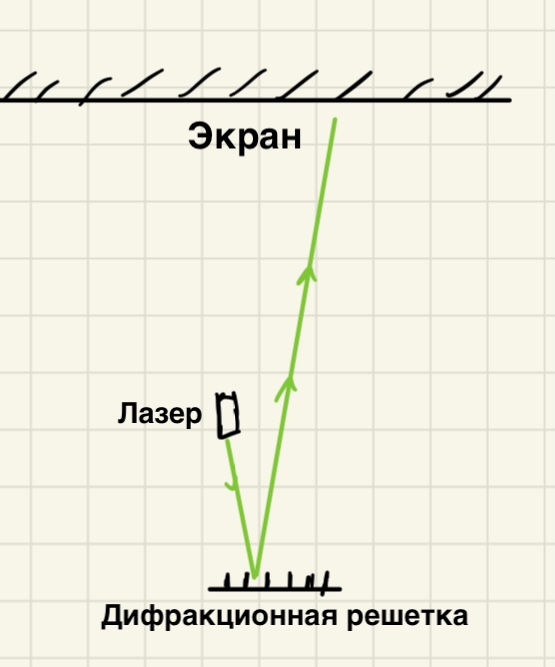
\includegraphics[width=0.5\textwidth]{setup}
\caption{Экспериментальная установка (вид сверху)}
\end{figure}

Схема используемой в работе экспериментальной установки изображена на Рис. 5. Луч лазера  падает на держатель с исследуемой решёткой, дифракционная картина в результате отражения наблюдается на экране с предварительно закреплённым на нём листом миллиметровой бумаги. Число облучаемых лазером полос $N \approx 25$.

Полученные дифракционные картины представлены на фотографиях ниже (см. Рис. 6, 7).

\begin{figure}[h!]
\centering
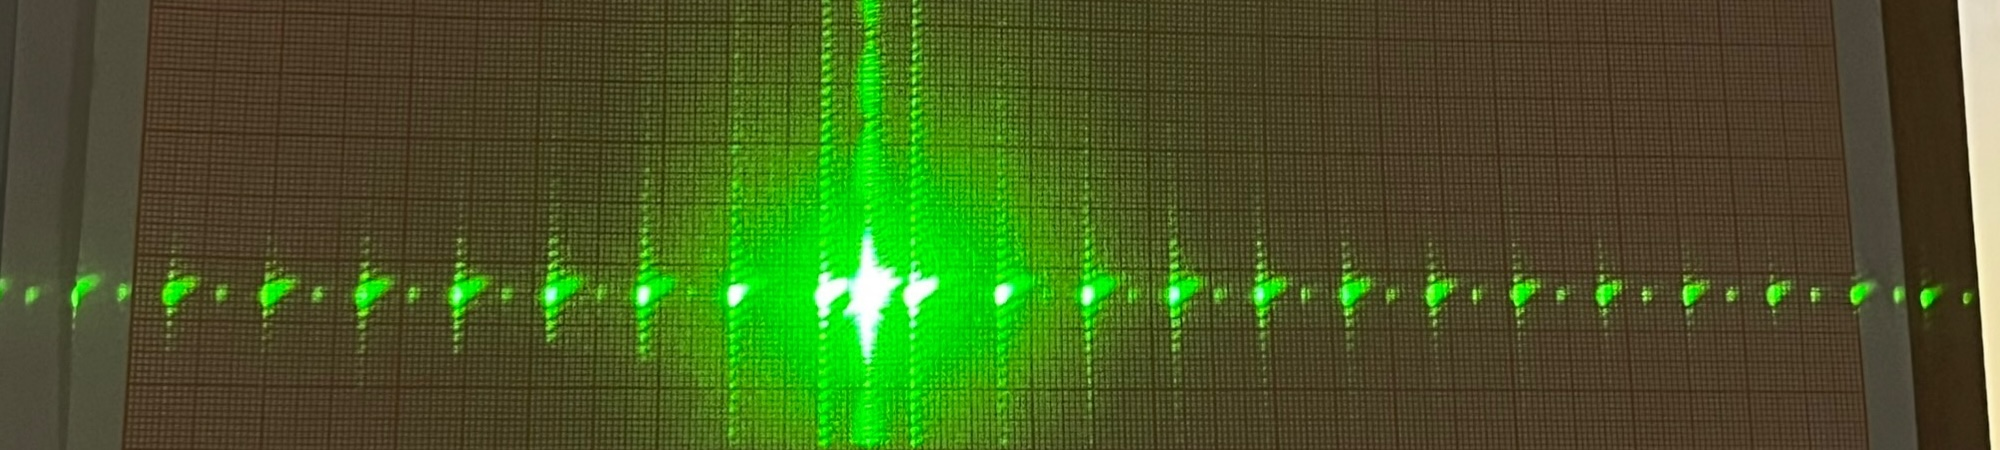
\includegraphics[width=0.8\textwidth]{ox}
\caption{Дифракционная картина для решётки на чистой подложке}
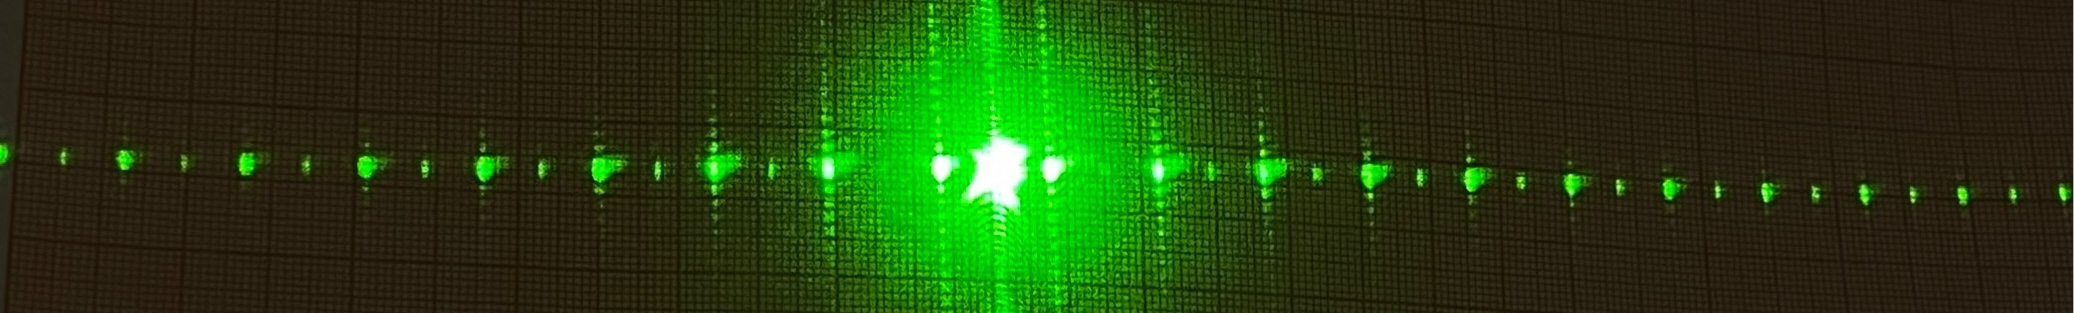
\includegraphics[width=0.8\textwidth]{unox}
\caption{Дифракционная картина для решётки на оксидированной подложке}
\end{figure}

\section*{Обработка экспериментальных данных}
Как было сказано ранее, интенсивность света как функция угла $\phi = \frac{x}{L}$, отсчитанного от нормали к плоскости решетки, равна:
\[
I = \left( \frac{\sin(\pi b \sin(\phi)/\lambda)}{\pi b \sin(\phi)/\lambda} \right)^2 \cdot \left( \frac{\sin(N\pi d \sin(\phi)/\lambda)}{\pi d \sin(\phi)/\lambda} \right)^2
\]
Первый множитель в этом выражении описывает огибающую (sinc), второй позволяет получить условие на главные максимумы: $d \sin(\phi) = m\lambda$. Поскольку расстояние между главными максимумами $x \ll L$, можно считать $\sin(\phi) \approx \phi = \frac{x}{L}$. Таким образом, измеряя положения главных максимумов $x$, можно получить длину волны лазера из коэффициента $k$ линейной зависимости:
\begin{align*}
	x=kn && \lambda=k\frac{d}{L}
\end{align*}

\begin{figure}[H]
\centering
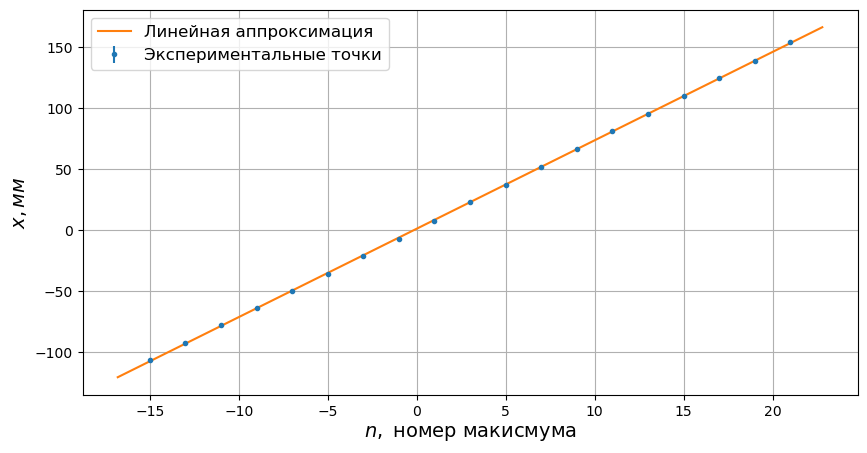
\includegraphics[width=0.9\textwidth]{unox_plot.png}
\caption{Линейная аппроксимация для решетки на чистой подложке (главный максимум - нулевой)}
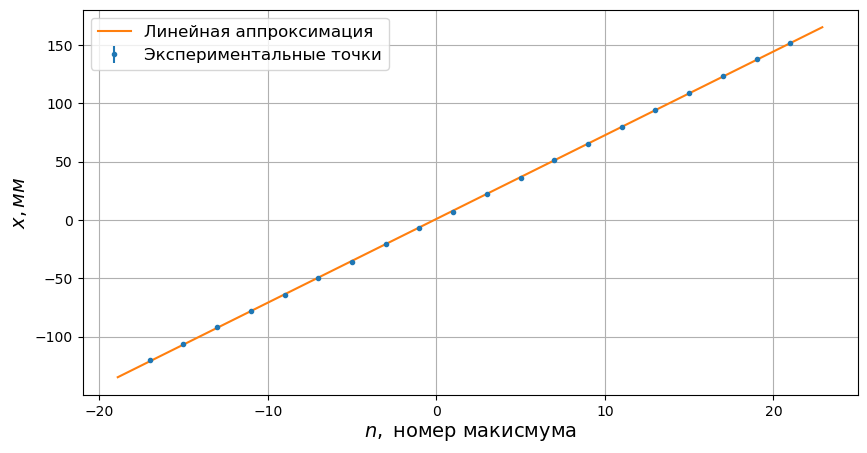
\includegraphics[width=0.9\textwidth]{ox_plot.png}
\caption{Линейная аппроксимация для решетки на оксидированной подложке}
\end{figure}

Измеренные ранее значения величин $d$, $L$, $x$, а также их погрешности представлены в таблице ниже. Расстояние от исследуемой решётки до экрана было измерено сантиметровой рулеткой. Положение максимумов определялось по милллиметровой бумаге с погрешность $\Delta x =1$ мм
\begin{table}[H]
\centering
\caption{Расчёт длины волны лазера}
\begin{tabular}{ccc}
\toprule
Величина & Чистая подложка & Оксидированная подложка \\
\midrule
$d$, мкм & $200.5 \pm 1$ & $200.3 \pm 1$ \\
$L$, см & $270.3 \pm 0.5$ & $270.5 \pm 0.5$ \\
$k$, мм & $7.243 \pm 0.014$ & $7.177 \pm 0.012$ \\
$\lambda$, нм & $537.2 \pm 1$ & $531.4 \pm 0.9$ \\
$\sigma_\lambda$ & 0.2\% & 0.2\% \\
\bottomrule
\end{tabular}
\end{table}

Как можно заметить, полученные результаты для двух решеток серьезно отличаются, вероятно это связано с общей хлипкостью установки и прочими случайными неточностями. Дополнительно, используемая теоретическая модель опирается на нормальное падение луча на решетку, что недостижимо на нашей установке (но необоходимо стараться делать угол наименьшим).

Наибольший оценимый вклад в погрешность каждой решетки вносит измерение диффракционной картины по миллиметровки, для увеличения точности стоит применить более точный способ детектирования. 


\section*{Анализ результатов работы}
В ходе работы были изготовлены образцы дифракционные решетки на подложках из чистого и оксидированного кремния, полученные с использованием метода контактной литографии. С помощью оптической микроскопии были измерены параметры изготовленных решёток, их отличие от использованного дизайна составило порядка 1\%.

Эксперимент по измерению волны лазера дал результат, близкий к ожидаемому. Наибольшая слабость этого эксперимента состоит в неустойчивости всех держателей, которые проявились в существенном отличии полученных значений для двух решеток. Для улучшения измерений стоит проводить их на оптическом столе с стандартными держателями, далее применить другой метод фиксации дифф картины. Итого, длина волны лазера:
\begin{align*}
	\lambda=534\pm3 ~\text{нм} && \sigma_\lambda=0.6 \%
\end{align*}

Полученные в результате эксперимента дифракционные картины совпали с результатами распределения интенсивностей, предсказанными теоретически и визуализированными при помощи компьютерного моделирования.
\newpage
\section*{Приложение}

\begin{figure}[h!]
\centering
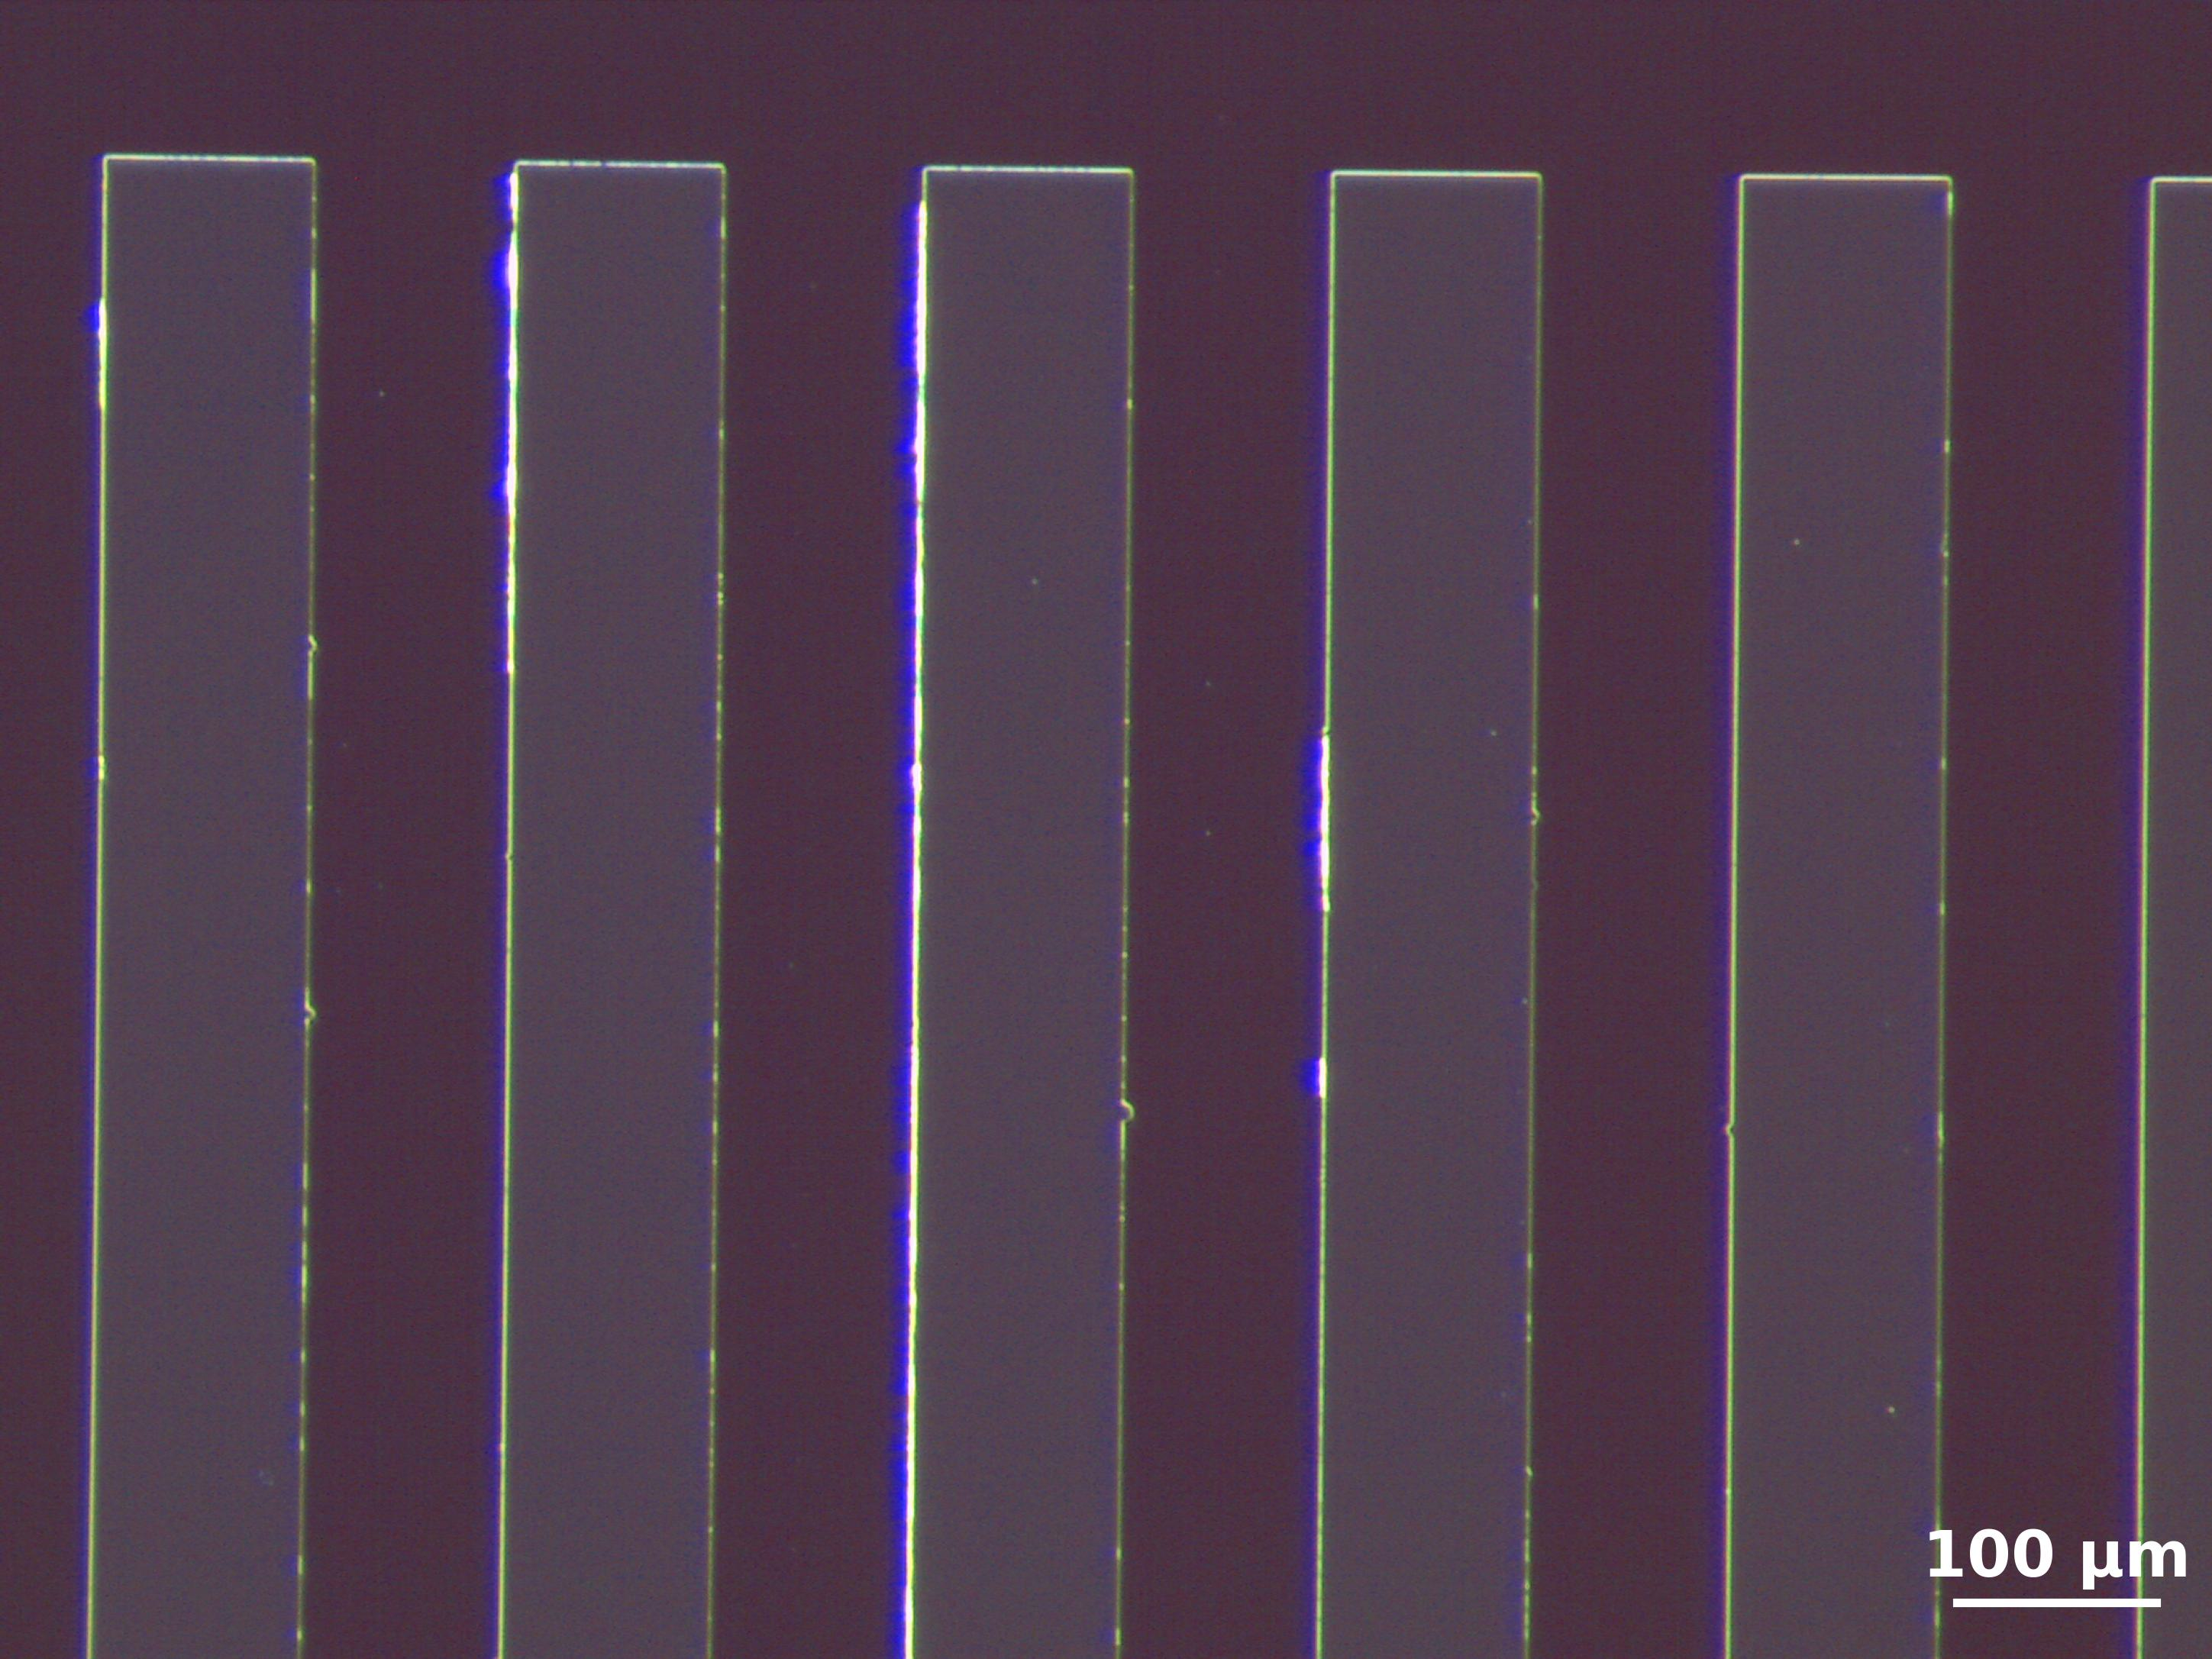
\includegraphics[width=0.8\textwidth]{unox_opt_scale.jpeg}
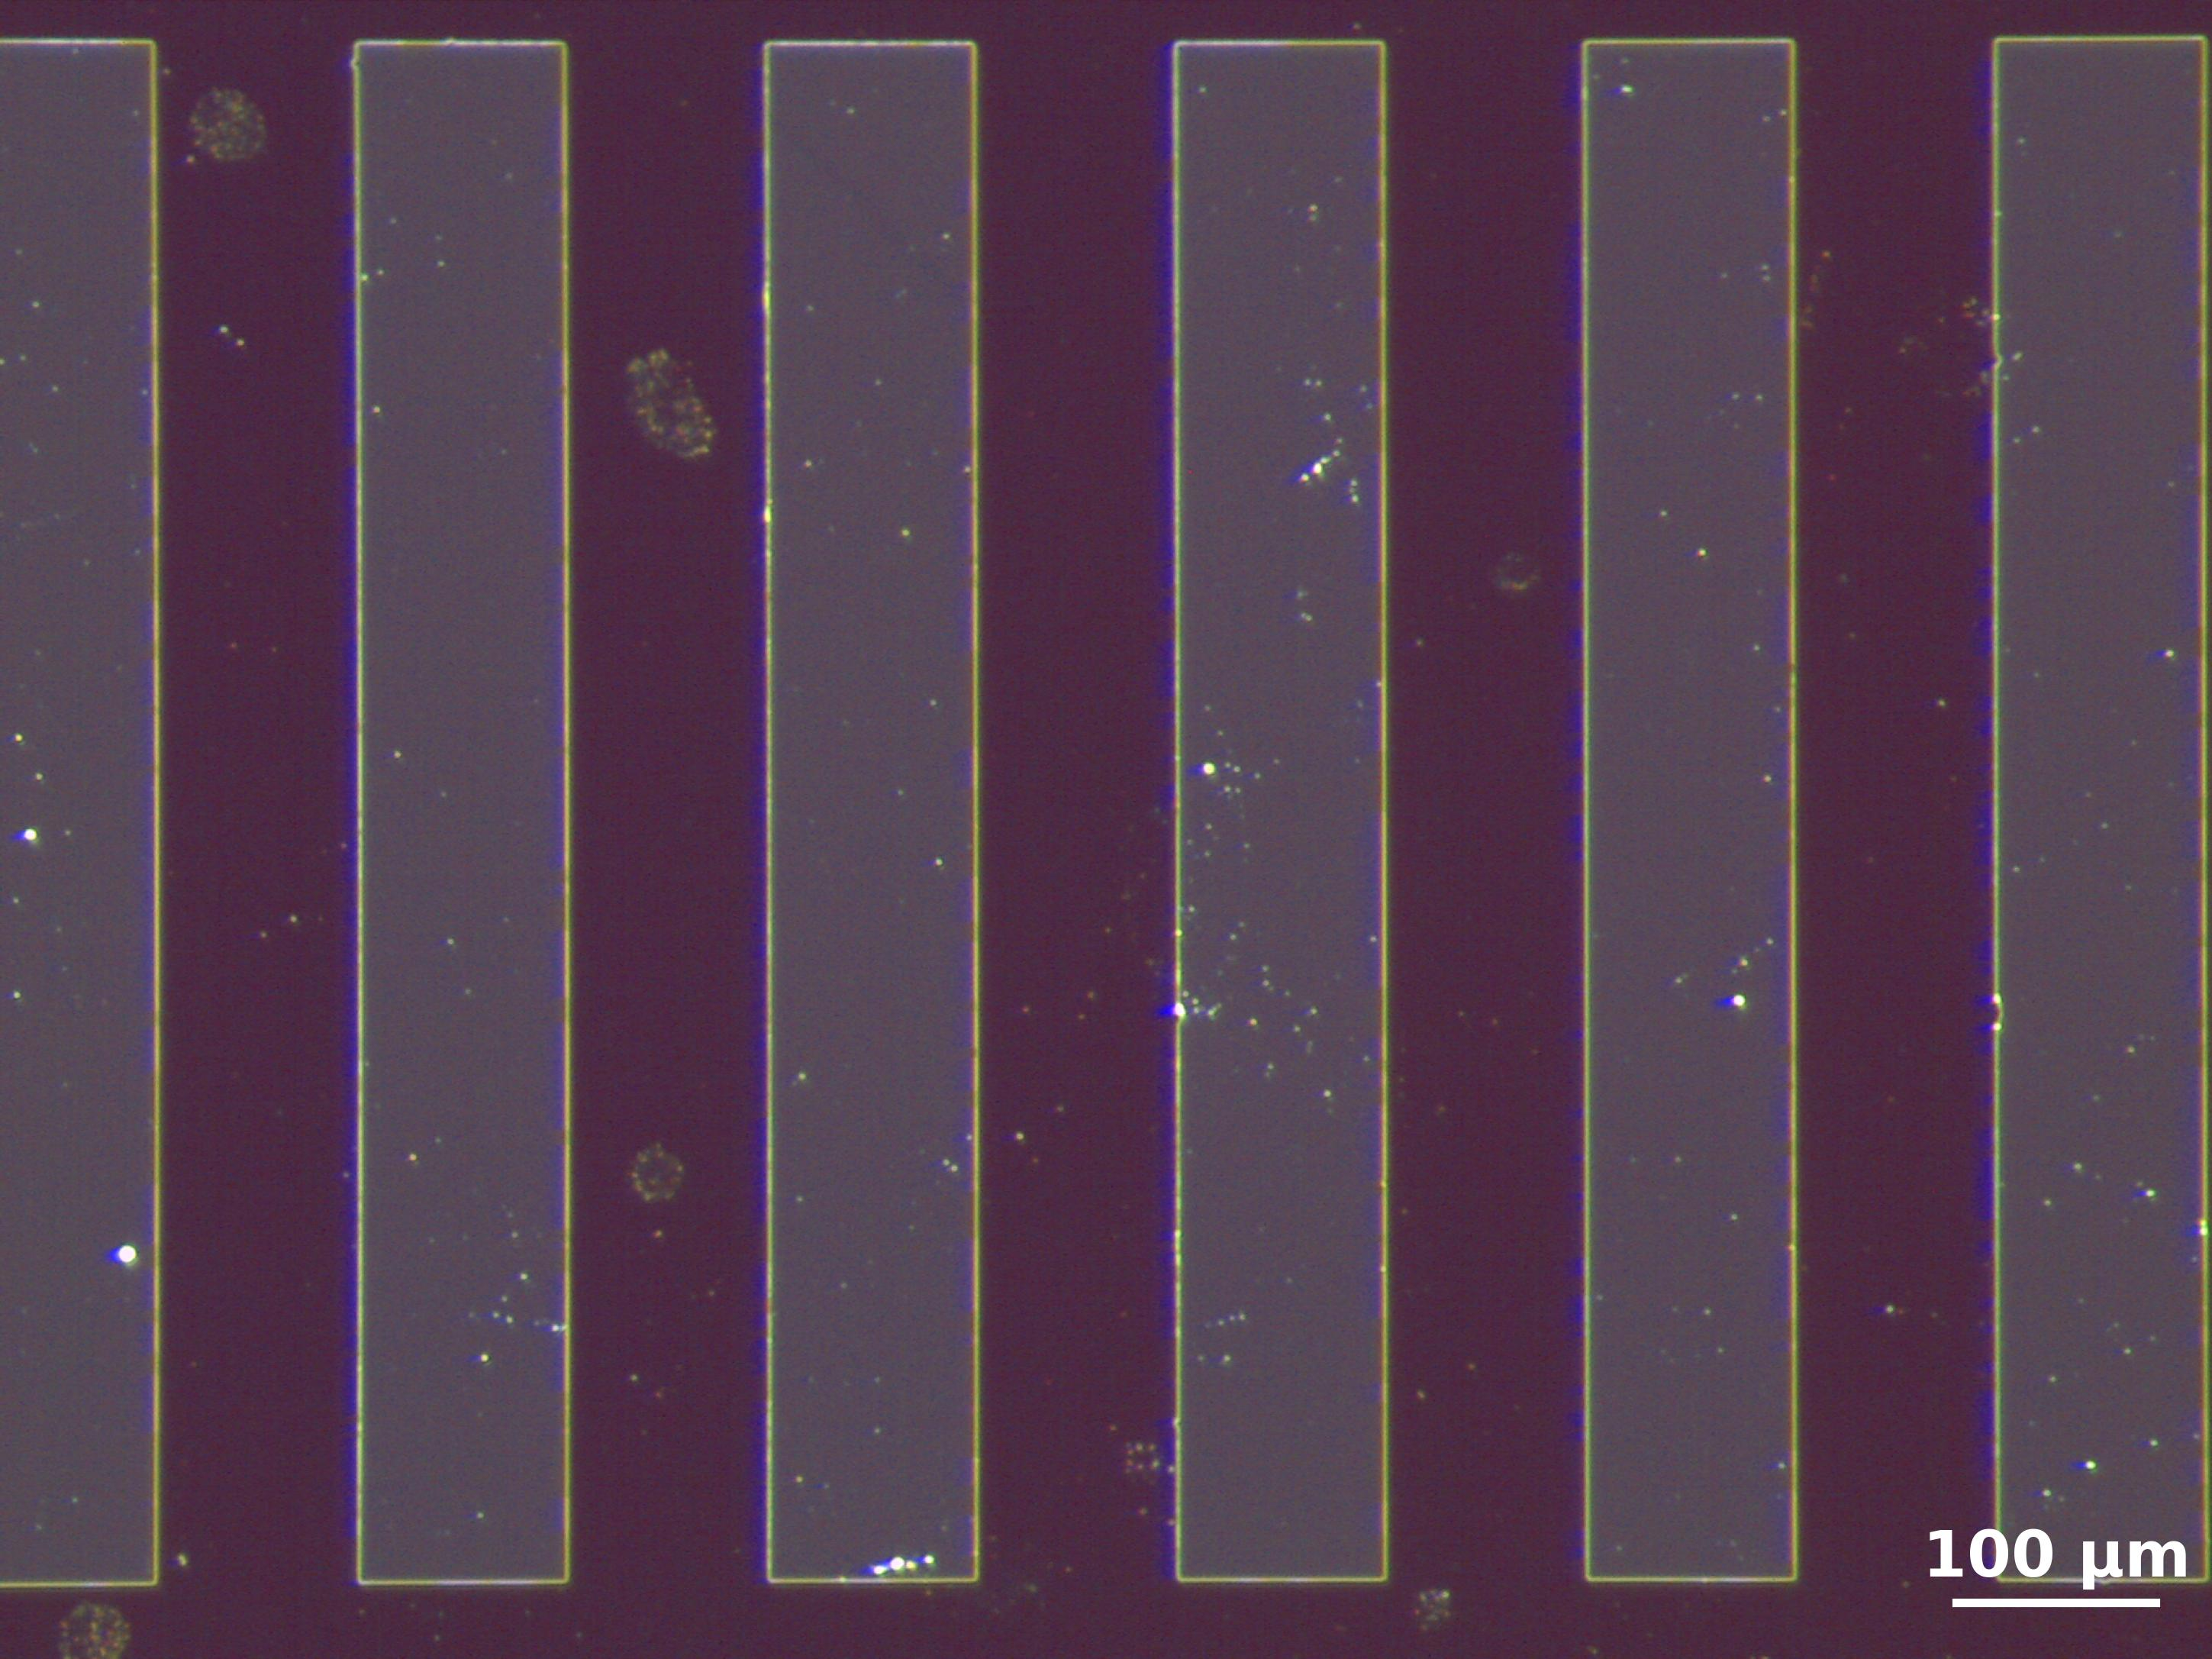
\includegraphics[width=0.8\textwidth]{ox_opt_scale.jpeg}
\caption{Изображения изготовленных образцов в оптическом микроскопе: сверху – на кремниевой подложке, снизу – на оксидированной. Измерения параметров дифракционных решёток проводились по этим изображениям}
\end{figure}

\begin{figure}[h!]
\centering
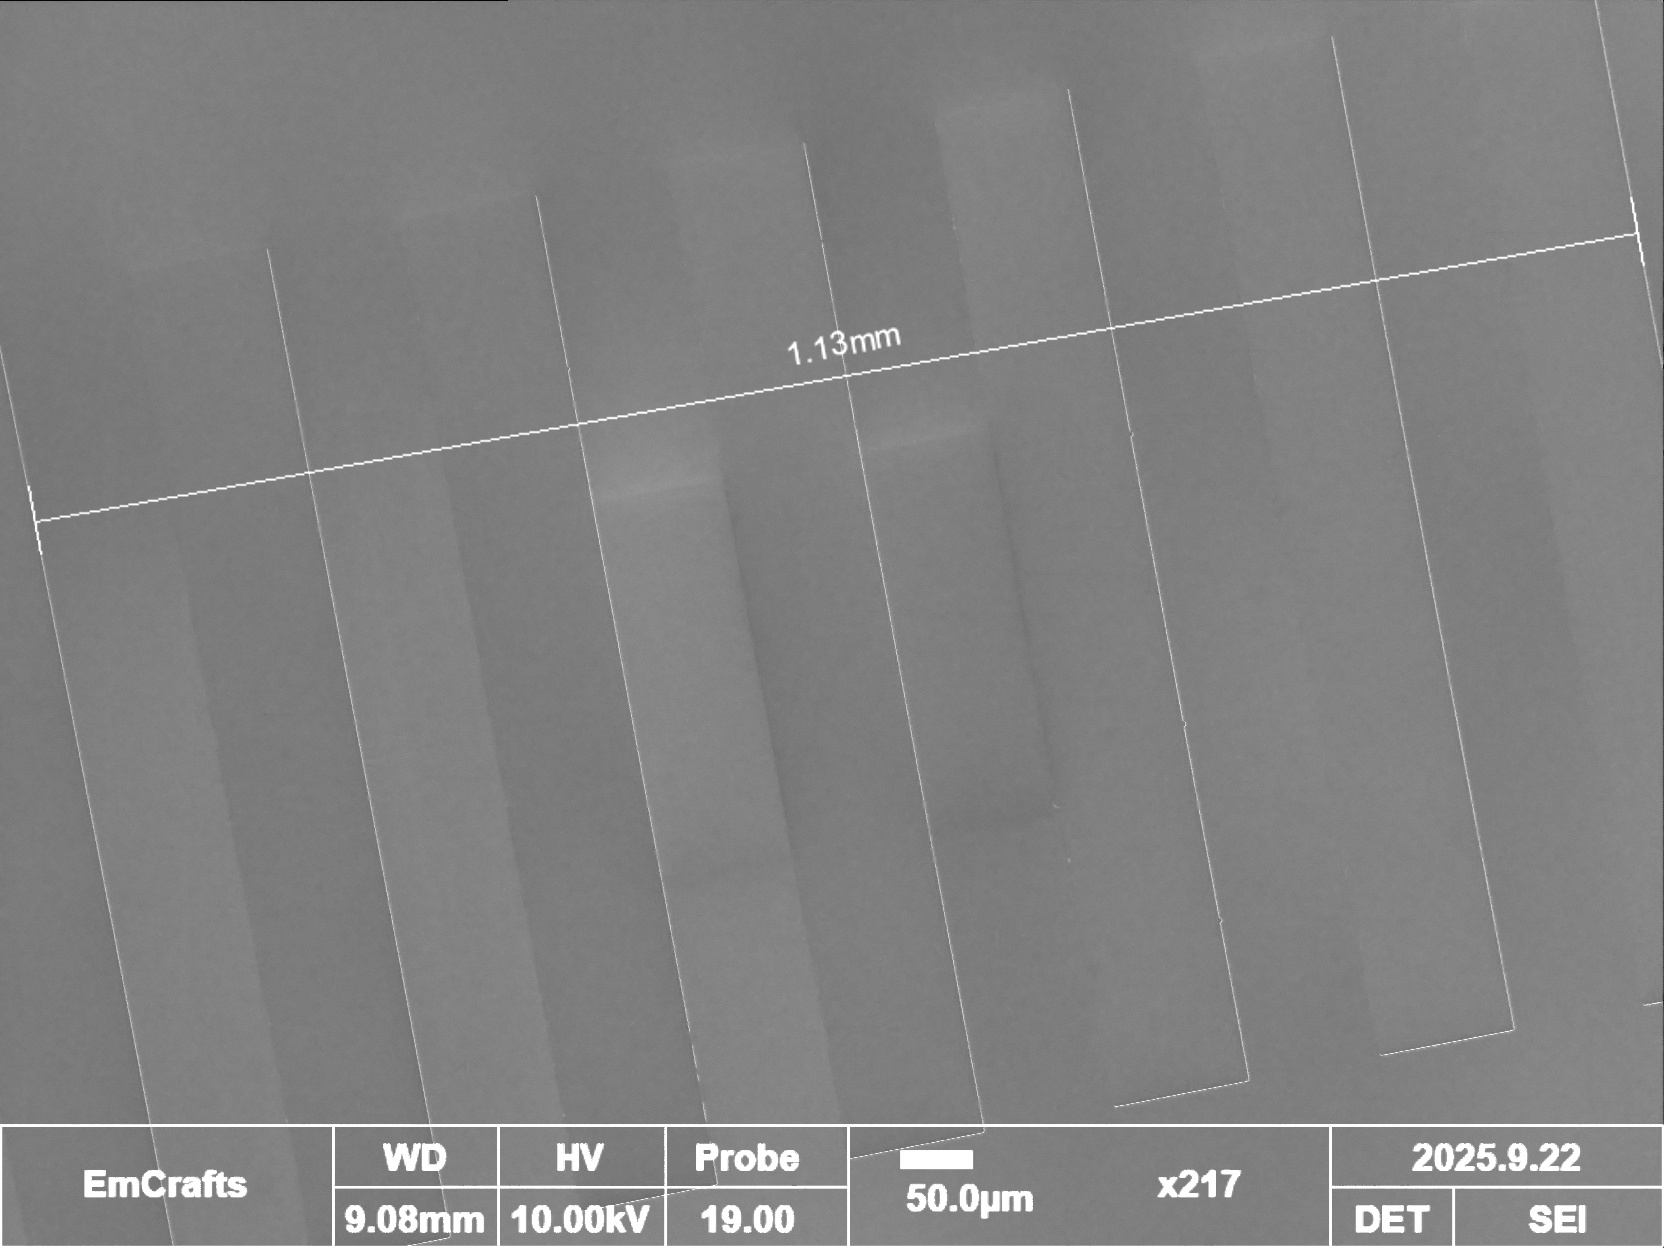
\includegraphics[width=0.8\textwidth]{sem_small}
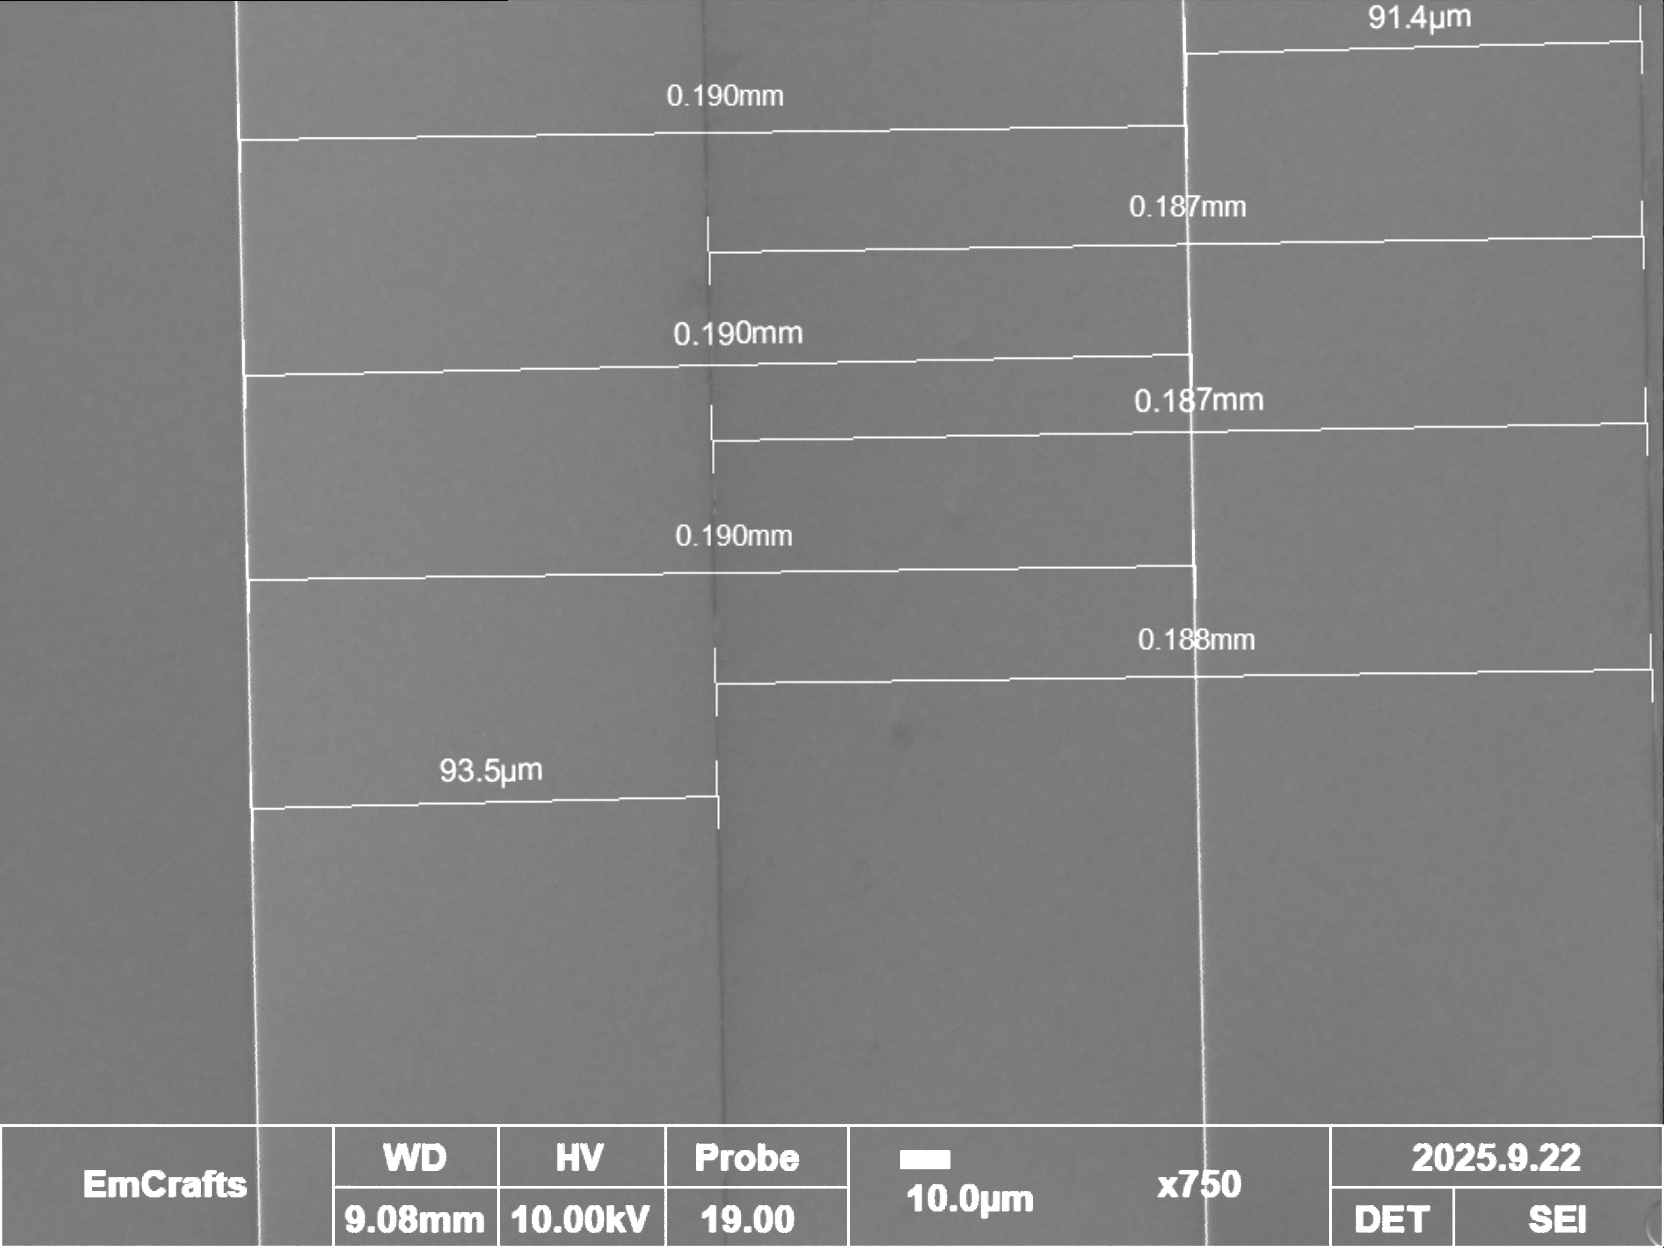
\includegraphics[width=0.8\textwidth]{sem_big}
\caption{Изображение решетки на чистой подложке полученное с помощью сканирующего электронного микроскопа}
\end{figure}

\end{document}
